% openany makes chapters start on even pages too
\documentclass[openany, 12pt]{book}

% sets margins of text inside page to 1 inch
\usepackage[top=1in, bottom=1in, left=1in, right=1in]{geometry}

% this will indent the first paragraph in a chapter
\usepackage{indentfirst}

% to use href
\usepackage{hyperref}

% to use images
\usepackage{graphicx}
% where images are stored
\graphicspath{{images/}}

\title{
  Introduction to Fitness \\
  \vskip 0.5cm
  \small A Technical Book on Fitness}
\author{Mihail Dunaev}
% this will remove date
\date{}

\begin{document}
  \maketitle
  \tableofcontents

  \chapter{Introduction}
  
	I have no background in fitness or nutrition. In school I studied Computer Science and now I work as a Software Engineer. What made me get more 
	into fitness was my weight: I was fat. Multiple times in my life. First, growing up as a kid I was fat and I managed to lose the weight in 
	secondary school just by eating less. Second time I got fat was in university, just because I lacked any motivation to study for exams and would
	power my way through with food and energy drinks. After uni I found it much harder to lose weight than I previously knew. I would follow a lot 
	of diets (keto\footnote{\href{https://en.wikipedia.org/wiki/Ketogenic_diet}{Ketogenic Diet on Wikipedia}}, food replacement like 
	soylent\footnote{\href{https://en.wikipedia.org/wiki/Soylent_(meal_replacement)}{Soylent on Wikipedia}} or 
	huel\footnote{\href{https://en.wikipedia.org/wiki/Huel}{Huel on Wikipedia}}), sometimes going really low in calories intake, feeling like I 
	have no energy and gaining the weight back on after ending the diet. I needed a better solution to this: I decided to start going to the gym.
	
	I guess my goal was to build muscle and lose fat. I've always liked muscles as a kid, just never got the time to look into it and start
	working out. This was my chance. I had a lot of questions: how do I train? What do I eat? Are there other things I need to pay attention to?
	One solution would be to hire a personal trainer to help me achieve this goal. What stopped me from doing this is the way my brain works: I knew
	I would just be given a list of things to do without any explanation. I really like to understand how things work and I would end up being 
	disappointed. This is also a big part of my life by now, I definitely wanted to understand well how everything works. I started looking into fitness
	the same way I look into everything: start searching on google, looking at professional bodybuilders, what they say, does it make sense etc. 
	I feel that if you want to know a subject really well you should look for competitions related to that subject, and see what the people involved
	have to say about it. This is why I started following people that compete in bodybuilding shows, strongman competitions and so on. 	
	What bothered me was how poorly organised the fitness information I found was. I couldn't find a single place that could take me from 0 knowledge
	to getting started in a matter of few hours. I had to watch a lot of youtube videos, read a lot of articles and posts in fitness communities until
	things were clear in my head. Now that I know all this information I think it's possible to put it all in one place: this is the purpose of this 
	book, to get you started with your fitness journey, especially if your goal is to build muscles and lose fat. And as I understand, this is the case
	for	most people working out.
	
	I just want to stress out: there is nothing wrong with being fat. If you get really fat it is unhealthy and you'll end up with 
	health problems. However, the main reason I don't want to be fat is because I get anxiety from it. I feel like crap, especially if I take my shirt 
	off in public. Saying I don't care about it is just lying to myself and I try my best to not do that, just for my mental health. This anxiety is
	something I can't control so for me the only solution would be to stay in shape. Besides, I already said I like muscles, so becoming muscular would
	make me feel proud of myself.
	
	The book is structured in two parts: nutrition \& workout. There is a lot of information in here, you don't necessarily need to understand all of it
	to get going. That's why at the end I just added an example of everything I did to get in my current shape without extra explanations. I will try 
	my best to present information in an unbiased way, presenting what people think works and what not, what I tried on myself etc. If you think 
	something is wrong or don't agree with some of the information presented here, this is an open source book so feel free to submit a 
	PR!\footnote{\href{https://docs.github.com/en/free-pro-team@latest/github/collaborating-with-issues-and-pull-requests/about-pull-requests}
	{About Pull Requests on Github Docs}} At the end of the day I am a practical person, I only believe in results and what works in real life. 
	I can say that the information I describe in this book worked really well on me, as you can see in the picture below.
	
	\begin{figure}[h]
		\centering
		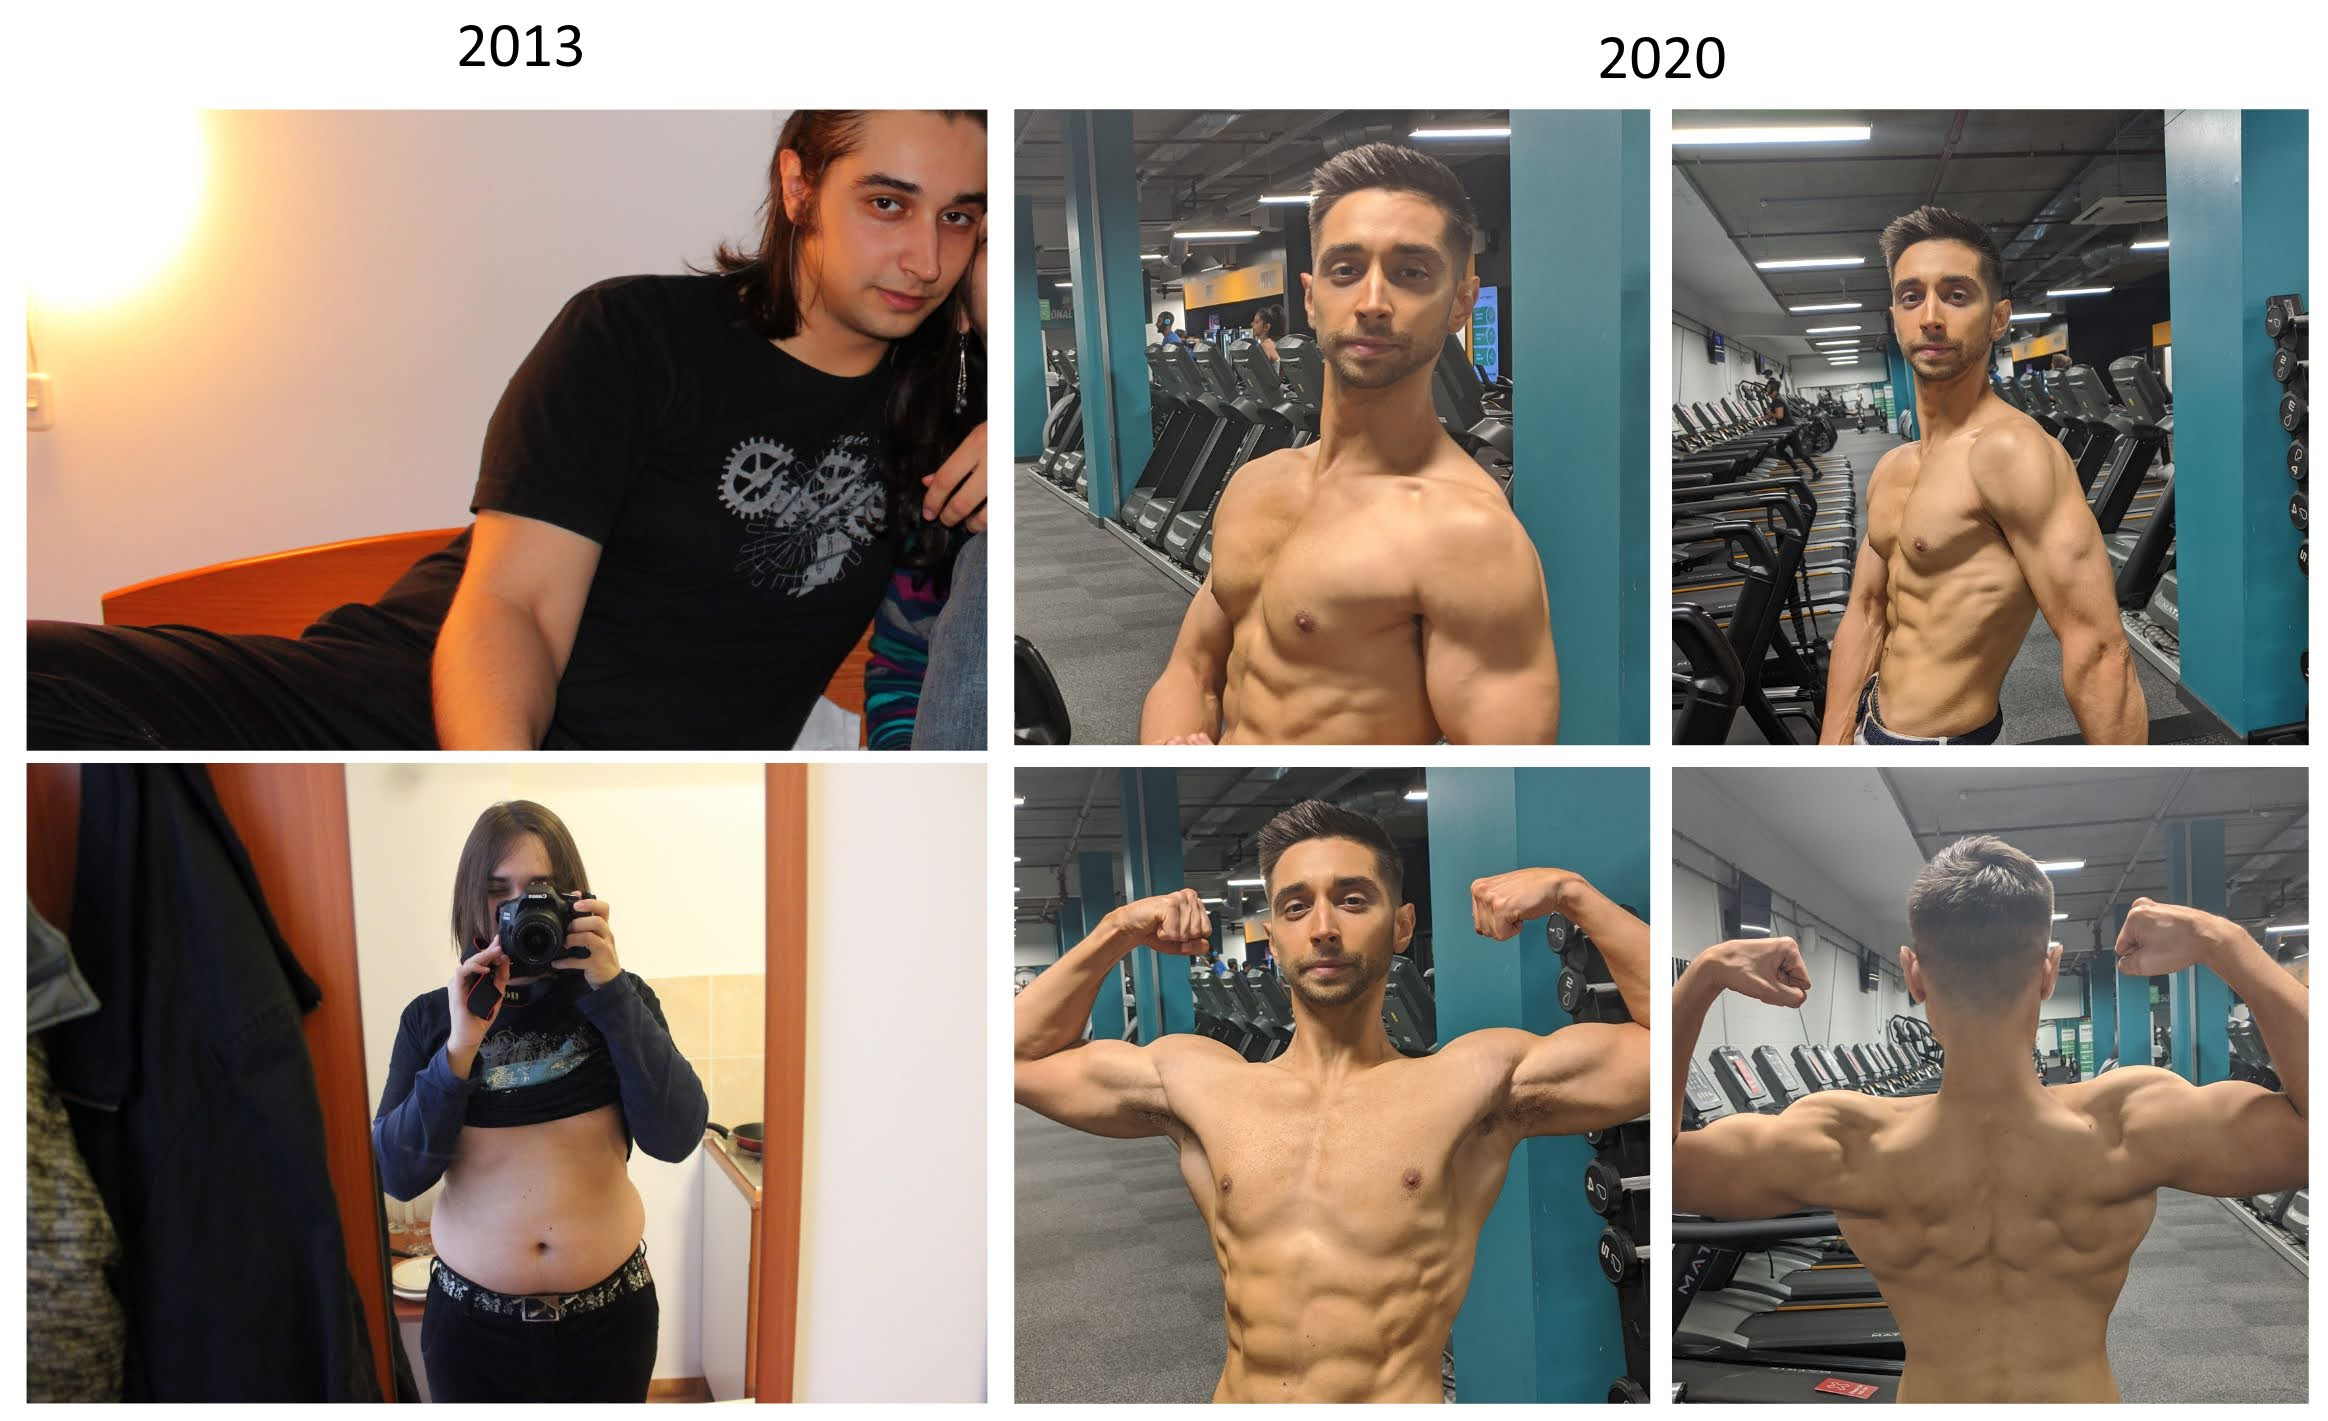
\includegraphics[scale=0.2]{transformation.jpg}
		\caption{From fat to muscular in 7 years: my lifelong struggle with being fat}
		\label{fig1}
	\end{figure}
	
	
  \chapter{Nutrition}
  
  	\section{Calories, BMR, TDEE}
  	
	I feel like I need to explain how food works first before anything else. Your body is an energy convertor. It gets energy from food\footnote{\href{https://en.wikipedia.org/wiki/Food_energy}{Food Energy on Wikipedia}} and converts it to heat, movement (kinetic energy) and 
	electrical energy for thinking. The amount of energy needed without movement (so for heat, thinking and perhaps others things too) is referred 
	to as basal metabolic rate or BMR\footnote{\href{https://en.wikipedia.org/wiki/Basal_metabolic_rate}{Basal Metabolic Rate on Wikipedia}} and it
	doesn't change much from day to day. If you include the energy for movement too you get your total daily energy expenditure or TDEE. If you eat
	more than your TDEE in a day, the extra food will be stored on your body either as fat or muscle. If you eat less then your body will have to go
	to fat stores and muscles and break them down to get the extra food energy you need. Energy is measured in $kcal$, but most of the time you will
	only see the term calorie with the same meaning (basically $kcal$ is the scientific term which was replaced by calorie when it started being used
	by food industries). To put energy values into perspective, the average human would need 2,000 calories for heat every day, or so I've seen in a
	physics course a long time ago. If I run on the treadmill for 1h I get a message that I burned roughly 600 calories. 1 Big Mac has almost 600 calories.
        It's important to understand that knowing exactly how many calories a meal has is next to impossible. There will always be small differences in every
        ingredient you use. For example not all loafs of bread are the same size, not all strawberries contain the same amount of sugar and so on. It's also
        impossible to know exactly how much energy you burn in a day. However, estimates work really well in practice. As long as you eat the same meals every week,
        you will either lose, gain or maintain weight.
	
	People have tried to come up with formulas to compute BMR from different factors, such as height, age, sex or body fat percentage (this is just
	the proportion of fat you have in your body relative to your whole mass, so 100 $\times$ fat mass / body mass). At first only mass (m), height (h) 
	and age were taken into account in Harris-Benedict formula for BMR from 1919\footnote{\href{
	https://en.wikipedia.org/wiki/Harris\%E2\%80\%93Benedict_equation}{Harris-Benedict on Wikipedia}}
	\begin{equation}
		BMR = 13.7516m + 5.0033h + 66.4730
	\end{equation}
  	This formula was later revised in 1984 with just a few minor changes. Later in 1990 Mifflin St Jeor\footnote{\href{https://pubmed.ncbi.nlm.nih.gov/2305711/}{A new predictive equation for resting energy expenditure in healthy individuals (1990)}} came with 2 formulas for BMR, one for men (\ref{males}) and one for women (\ref{females}).
	\begin{equation}
		\label{males}
		BMR (males) = 10m + 6.25h - 5a + 5
	\end{equation}
	\begin{equation}
		\label{females}
		BMR (females) = 10m + 6.25h - 5a - 161
	\end{equation}
	Finally Katch-McArdle\footnote{\href{https://books.google.co.uk/books/about/Essentials_of_Exercise_Physiology.html?id=L4aZIDbmV3oC}{Essentials of Exercise Physiology Book by Katch \& McArdle (2006)}} included body fat percentage (f) into the equation, removing age and height
	\begin{equation}
		BMR = 370 + (21.6m (1 - \frac{f}{100}))
	\end{equation}
	This is an interesting point because body fat percentage does affect how many calories you burn even at rest. The rule I know is that 10 pounds of muscle would burn 50 kcal in a day at rest, while 10 pounds of fat will only burn 20 kcal\footnote{\href{https://www.webmd.com/diet/obesity/features/8-ways-to-burn-calories-and-fight-fat}{Burning Calories on WebMD}} (less than half), so if you're 80kg with 15\% body fat you will burn more calories at rest than someone who is 80kg with 20\% body fat. This also explains the Mifflin St Jeor above, since women have naturally more fat than men. 
	
	Let's take an example using the last formula: if you weight $70kg$ and your body fat percentage is $18\%$ then your BMR should be $370 + (21.6 \times 70 \times (1 - 18/100)) = 1609.84$ calories. Add your movement energy to this and you get your TDEE. I haven't spent the time trying to derive how to
	compute this one (e.g. from kinetic energy) because all of these formulas are great but at the end of the day they are just for your orientation.
	The best way to compute your TDEE is to actually measure it: without changing your habits, eat 2,000 calories every day for 1-2 weeks. Weight
	yourself every day: does your weight change? If no then it's safe to assume your TDEE is 2,000 calories. Does your weight go up? It probably means
	your TDEE is lower. Keep adjusting your calories intake until you find your TDEE. 
	
	In theory you should be able to tell your TDEE without having
	to change your diet again just by looking at how much weight you gained / lost in the initial 1-2 weeks: you should lose 1lb (or 0.45kg) of mass at 
	a total deficit of 3500 calories\footnote{\href{https://www.ncbi.nlm.nih.gov/pmc/articles/PMC2376744/}{What is the Required Energy Deficit per 
	unit Weight Loss? (2008)}}. Let's take an example again: you ate 2,000 calories for 2 weeks. During these 2 weeks you gained 2.2lbs (or 1kg) on the
	scale. According to the 3500 rule, you were at a total surplus of $3500 \times 2.2 = 7700$ calories. This surplus was achieved in 14 days, so the
	surplus each day was 550 calories. This means your actual TDEE is 2,550 calories. However I found this rule to not work on me, trying to adjust 
	accordingly didn't put me at maintenance and I kept changing weight. As long as you always adjust to results you will be fine. I would personally
	start with an online TDEE calculator\footnote{\href{https://tdeecalculator.net/}{Example of online TDEE calculator}} (there are plenty out there) 
	just to get a value to work with, then keep adjusting intake until I hit my maintenance.
	
	
	\section{Body Fat Percentage}
	
	Body fat percentage is discussed a lot in fitness because it affects how you look. Fat is something that is stored on your body between skin and muscles. The more fat you have on you the less visible your muscles will be. However, just taking the absolute value of fat mass is not a good indicator of how well your muscles are showing, since taller people will have more fat mass but more body surface to spread it across. So instead we can look at the proportion of fat in relation to muscles. The body fat percentage will normally dictate certain features you can see on your body, for example the average guy will have his abdominal muscles ("abs") showing around 10-14\% body fat\footnote{\href{https://www.healthline.com/health/body-fat-percentage-for-abs}{Healthline Article on Abs}}. To better understand what I'm talking about look at the image below that I found on builtlean.com\footnote{\href{https://www.builtlean.com/body-fat-percentage-men-women/}{Body Fat Percentage Photos Of Men \& Women}}. I cannot confirm the numbers to be correct but they give a good indication in my opinion to what body fat percentage looks like at different values (note that lower body fat percentage will not give you bigger muscles, it just happens to be the case in the pictures).
	
	\begin{figure}[h]
		\centering
		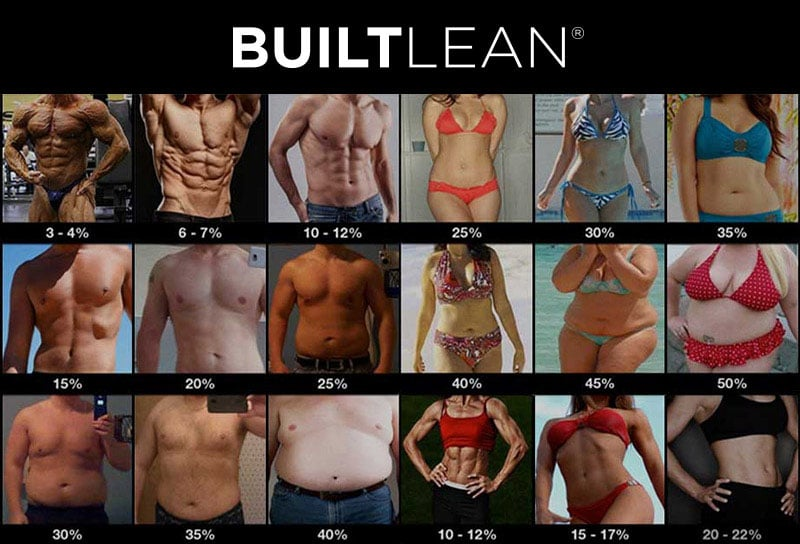
\includegraphics[scale=0.6]{bodyfatpercentage.jpg}
		\caption{Different body fat \% for both men and women}
	\end{figure}
	
	Computing body fat percentage is not easy. There is no 100\% accurate way of doing it. You can take pictures of yourself in the mirror and then compare with the images above, a lot of people estimate this way and I find it good as well. If you want a more accurate way of doing it though, there are a few options out there. The most accurate way is an MRI scan\footnote{\href{https://pubmed.ncbi.nlm.nih.gov/9655763/}{Cadaver validation of skeletal muscle measurement by magnetic resonance imaging and computerized tomography}}. However this is not available to the public as far as I know. This leaves us with the second most accurate option I know, which is a DEXA scan\footnote{\href{https://en.wikipedia.org/wiki/Dual-energy_X-ray_absorptiometry}{DEXA on Wikipedia}}. This is a machine that does an x-ray scan of your body. It shows quite some details, for example the lean mass and fat mass in your arms, trunk (core) and legs. You can see an example of a DEXA scan result below.
	\begin{figure}[h]
		\centering
		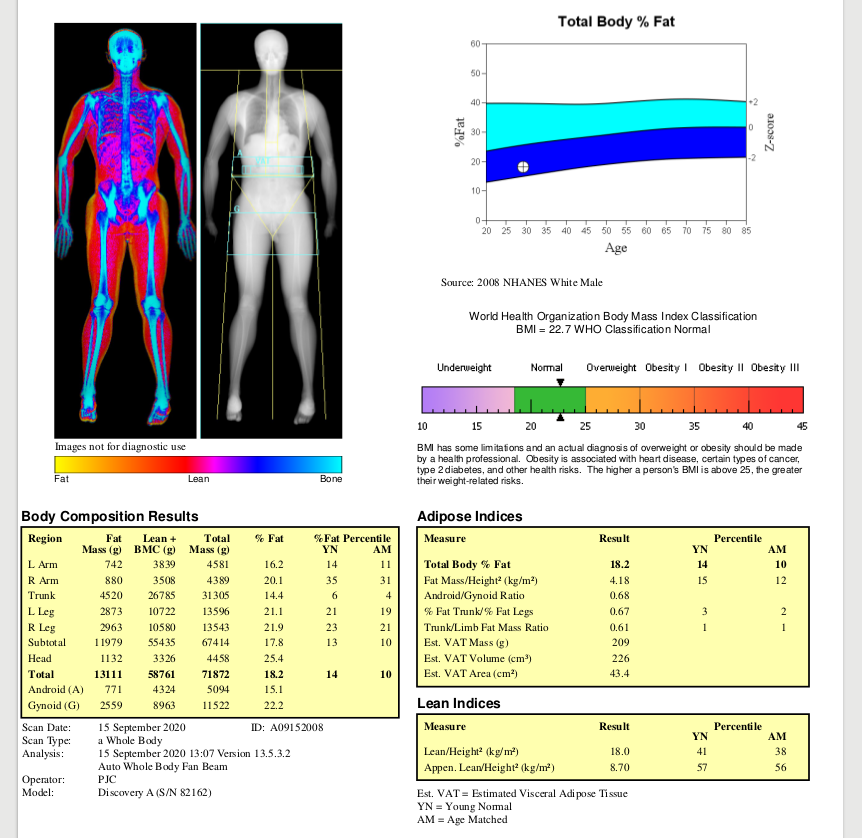
\includegraphics[scale=0.5]{dexa-scan.png}
		\caption{Result of a DEXA scan, showing body fat for different body parts}
	\end{figure}
However, DEXA scans can have errors too, and a lot of people talk against it\footnote{\href{https://www.youtube.com/watch?v=2Gg4Jm5KS1Y}{Greg Doucette on DEXA Scans on Youtube}}\footnote{\href{https://www.youtube.com/watch?v=P17bcpYE8Ew}{Brain Shaw on DEXA Scans on Youtube}}. The scan is also expensive, I did it in London at bodyscan for roughly \pounds 100.
	
	Before DEXA scans, hydrostatic weighing\footnote{\href{https://en.wikipedia.org/wiki/Hydrostatic_weighing}{Hydrostatic Weighing on Wikipedia}} was considered the most accurate method available to the public. You had to step on a scale underwater and the value you get helps estimate your body density, which can be used to approximate your body fat percentage.	Another way of estimating body fat percentage which is similar to hydrostatic weighing is whole-body air displacement plethysmography\footnote{\href{https://en.wikipedia.org/wiki/Air_displacement_plethysmography}{Air Displacement Plethysmography on Wikipedia}} (for example Bod Pod\footnote{\href{https://www.cosmed.com/en/products/body-composition/bod-pod}{Bod Pod}}).
	
	More common methods of estimating body fat are the skinfold methods\footnote{\href{https://en.wikipedia.org/wiki/Body_fat_percentage\#Anthropometric_methods}{Skinfold Methods on Wikipedia}} (using a device called caliper) and using bioelectrical impedance analysis\footnote{\href{https://en.wikipedia.org/wiki/Bioelectrical_impedance_analysis}{Bioelectrical Impedance Analysis on Wikipedia}}. The first method tries to determine the thickness of the fat layer under the skin. You use the caliper at various spots on the body and look up the measurement in a table which will tell you the estimated body fat. It's best if you use a personal trainer or someone with experience to perform the reading. For bioelectrical impedance analysis a small electric current is sent through the body and the resistance of the whole body is computed, which depends on body fat percentage. Some scales also state they can compute body fat percentage just from your weight, height, age and sex. However this is not really possible unless you don't lift at all and the extra weight comes from fat alone. Just to recap all the methods described in this section, from most accurate to least one:
	
	\begin{enumerate}
		\item Magnetic Resonance Imaging (MRI) and Computerized Tomography (CT)
		\item Dual-energy X-ray absorptiometry (DEXA / DXA)
		\item Hydrostatic weighing
		\item Whole-body air displacement plethysmography
		\item Skinfold methods (calipers)
		\item Bioelectrical impedance analysis
	\end{enumerate}
	
	\section{Bulking \& Cutting}	
	
	Your TDEE is the total amount of energy your body needs every day to be able to function properly. If you eat less than that, your body has to go to fat stores or muscles to get that energy. If you eat more, the excess food will be stored on your body as fat or muscle. This is the reason people say that you need to be at a surplus to gain muscles, if you are at a caloric deficit then the proteins that should be stored on your muscles will be used for heat and movement instead. This phase in which you eat more than you should to build muscles is called bulking. Being at a caloric surplus will make it impossible for you to burn fat however, in fact you might end up gaining fat mass as well since the body is not optimal at storing pure muscles. To get rid of the excess fat you need to put yourself at a caloric deficit when you try to burn the fat stores while keeping the muscles you gained. This phase is called cutting. Bulking and cutting are normal cycles for bodybuilders, they will bulk, cut, bulk, cut and so on. There are instances when you can build muscles and cut down fat at the same time, I experienced this on myself when I started training again after a 3 months absence. I've read that it can also happen when you start training for the first time or if you take steroids, but more on steroids later. Building muscles and losing fat at the same time is also referred to as body recomposition\footnote{\href{https://www.healthline.com/nutrition/body-recomposition\#how-it-works}{Healthline Article on Body Recomposition}}.
	
	If you keep training (e.g. lifting weights) while cutting, your body will value your muscles more than the fat, so it will rather use fat to get the extra energy it needs. This is an oversimplified explanation of how everything works, in reality it's more complex than this. A different explanation would be this: the body has workers that take macronutrients (carbs, fat \& proteins) from food to places where they need to be. In this case the workers that take proteins to muscle is the testosterone in your body. Testosterone will race other workers that take macronutrients to produce heat and convert them to movement --- these workers prefer carbs and fat over protein. Based on how much testosterone you have and how easy it is for your body to rebuild the muscles you might be able to use all the proteins you get to gain muscles while the body will have to go to fat stores to get all the energy, so basically building muscles and losing fat at the same time. I've seen this analogy of testosterone with construction workers used a lot in fitness. 
	
	Knowing your TDEE, what is the caloric surplus you should aim for during a bulking phase? Most people seem to go 10-20\% more for what's considered a "lean bulk"\footnote{\href{https://www.youtube.com/watch?v=rCdba0UPTMk}{VitruvianPhysique on Lean Bulking on Youtube}}\footnote{\href{https://us.myprotein.com/thezone/nutrition/the-lean-bulk-how-to-minimize-fat-gain-while-bulking/}{Lean Bulk on Myprotein website}}. For example if your TDEE is 2,500 calories a day, you should eat 2,750 - 3,000 calories to lean bulk. If you go more than that it's considered a "dirty bulk" in which you gain more fat than you should. Doing a dirty bulk means you'll be spending more time to cut the fat afterwards. It can also make you feel like shit eating this much and dieting for so long. Sure it might give you more energy in the gym and make you even stronger (it's interesting how strength and muscle size are not perfectly correlated but more on this later) but it all depends on what you want to achieve. If you want to stay in shape all of the time then it's probably not for you, since the only time you'll be in shape is at the end of a cut for a short period of time. A lot of people speak against dirty bulks\footnote{\href{https://www.youtube.com/watch?v=DjEnkzhz5T4}{Greg Doucette on Bulking and Cutting on Youtube}}\footnote{\href{https://www.youtube.com/watch?v=xl0ZNFcvuJI}{Greg Doucette on Bulking on Youtube}} and I don't approve of them myself since I tried it once --- I felt like shit, out of shape and it made no sense to me since losing fat was one of the main reasons I got into this. You might also experience stretch marks on dirty bulks if you gain weight too fast\footnote{\href{https://www.bodybuilding.com/content/stretchmark-maintenance.html}{Article on Bodybuilding.com}}.
	
\end{document}
